%presentation
\documentclass{beamer}

%impressions
%\documentclass[handout]{beamer}
%\usepackage{pgfpages}
%\pgfpagesuselayout{2 on 1}[a4paper,border shrink=5mm]
%\setbeameroption{notes on second screen}
%\pgfpagelayout{2 on 1}[a4paper, border, shrink=5mm]
% vue sur http://wwwtaketorg/spip/articlephp3?id_article=30...
\usepackage[T1]{fontenc}
\usepackage[frenchb]{babel}
\usepackage[utf8x]{inputenc} % Pour pouvoir taper les accents sans faire de combinaison
%\usepackage{arev}
%\usepackage{aeguill}
%mode code
\usepackage{listings}

%mode verbatim
\usepackage{moreverb}

%\usepackage[darktab]{beamerthemesidebar}
%\leftsidebar
\usetheme{Hannover}
%\usetheme{Oxygen}
\usepackage{thumbpdf}
\usepackage{wasysym}
\usepackage{ucs}
\usepackage{pgfarrows,pgfnodes,pgfautomata,pgfheaps,pgfshade}
\usepackage{verbatim}


\title{Ruby, Ruby On Rails et le déploiement sur serveur d'application}
\author{Cyril Mougel}

\begin{document}

\section{Le langage Ruby}

\begin{frame}
	\frametitle{L'historique}
	\begin{itemize}
		\item Créé en 1993 par Yukihiro Matsumoto dit \og{}Matz\fg{} au Japon
		\item Langage de scripting Haut niveau où tout est objet
        \item Applique le principe de moindre surprise ( POLS, principle of
                least surprise)
        \item Fonctionne sur toutes les plateformes du marchés (Linux, Windows,
                Mac)
	\end{itemize}
\end{frame}

\section{Le concept de Ruby On Rails}


\begin{frame}
    \frametitle{Le framework Ruby On Rails}
    \begin{itemize}
        \item Créé par David Heinemeier Hansson dit \og{}DHH\fg{}
        \item Extrait de l'application BaseCamp de 37signals
        \item Premiere release public en 2004 
    \end{itemize}
\end{frame}

\begin{frame}
    \frametitle{Pourquoi Rails en Ruby ?}
    \begin{itemize}
        \item Multi-plateforme
        \item Forte facilité d'introspection et réflexion.
            \begin{itemize}
                \item User.findi\_by\_firstname\_and\_lastname 'David', 'Hanson'
                \item has\_many :galleries
            \end{itemize}
    \end{itemize}
\end{frame}

\begin{frame}
    \frametitle{Le concept de Ruby On Rails}
    \begin{itemize}
        \item Ruby On Rails conçu par des développeurs pour des développeurs
        \item Un cadre de travail minimal et complet pour un développement Web
        \item Convention over Configuration
        \item Don't Repeat Yourself (DRY)
        \item Say what you do, Do what you say
        \item Un seul et unique language pour tout faire
    \end{itemize}
\end{frame}

\begin{frame}
    \frametitle{Rails est MVC}
    \begin{itemize}
        \item Model : ActiveRecord
        \item View : ActionView
        \item Controller : ActionController
    \end{itemize}
\end{frame}

\begin{frame}
    \frametitle{Chaque chose à sa place}
    \begin{itemize}
        \item Chaque dossiers correspond à quelque chose et a son utilité
            propre
    \end{itemize}
    \begin{columns}
        \begin{column}[l]{4cm}
            \begin{figure}
                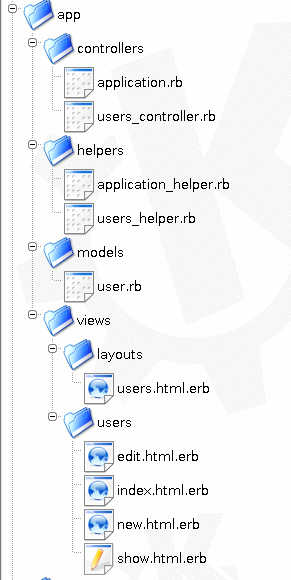
\includegraphics[width=30mm]{FS_1.png}
            \end{figure}
        \end{column}
        \begin{column}[r]{4cm}
            \begin{figure}
                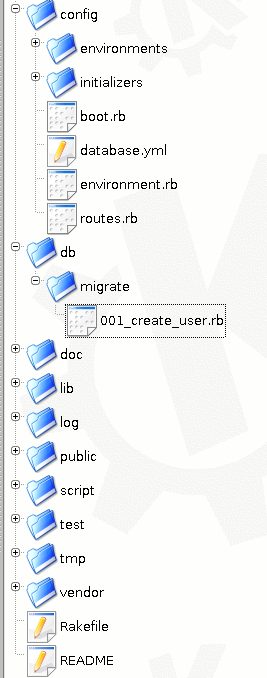
\includegraphics[width=25mm]{FS_2.png}
            \end{figure}
        \end{column}
    \end{columns}
\end{frame}

\section{Composant Model de Ruby On Rails}

\begin{frame}
    \frametitle{Gestion de la Base de donnée}
    \begin{itemize}
        \item Systeme de gestion de migration (ActiveRecord::Migration)
        \item Utilisation du pattern ActiveRecord
        \item Generation de nombreuses methodes utilitaires à la volée
    \end{itemize}
\end{frame}

\begin{frame}
    \frametitle{Migration de Base de donnée}
    \begin{itemize}
        \item Gestion incrémental des fichiers de migrations
        \item Retour avant arrière sur les migrations
        \item Utilisation de méthode Ruby au lieu de requête SQL pur
    \end{itemize}
\end{frame}
\begin{frame}
    \frametitle{Exemple de Migration}

    Voici donc un exemple de fichier de migration :


    \begin{center}
        \lstinputlisting[language=Ruby,basicstyle=\scriptsize,
        numbers=left]{066_fix_profiles.rb}
    \end{center}
\end{frame}

\begin{frame}
    \frametitle{La classe Mapping}
    Et pour la classe qui mappe notre classe Users qui possedent 6 champs~:
   
    \begin{columns}
        \begin{column}[l]{3cm}
            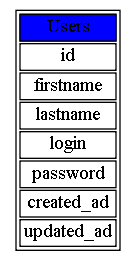
\includegraphics[width=20mm]{user.png}
        \end{column}
        
        \begin{column}[r]{10cm}
            \begin{block}{Code de la classe de Mapping}
              \lstinputlisting[language=Ruby,numbers=left,basicstyle=\scriptsize]{user.rb}        
            \end{block}
            \begin{block}{Exemple d'utilisation de la classe de mapping}
              \lstinputlisting[language=Ruby,numbers=left,basicstyle=\scriptsize]{user_use.rb}        
            \end{block}
        \end{column}
    \end{columns}

\end{frame}

\begin{frame}
    \frametitle{les méthodes static accessibles pour la classe User}
    Et bien-sûr toutes les méthodes accessible en static~:
    \tiny{}
    \begin{columns}
        \begin{column}[l]{6cm}
            \begin{itemize}
                \item User.find :all
                \item User.find\_by\_firstname 'Cyril'
                \item User.find\_by\_lastname 'Mougel'
                \item User.find\_by\_firstname\_and\_lastname 'Cyril', 'Mougel'
            \end{itemize}
        \end{column}

        \begin{column}[r]{6cm}
            \begin{itemize}
                \item User.count :all
                \item User.count\_by\_firstname 'Cyril'
                \item User.count\_by\_lastname 'Mougel'
                \item User.count\_by\_firstname\_and\_lastname 'Cyril', 'Mougel'
            \end{itemize}
        \end{column}
    \end{columns}
    \normalsize{}
    etc...
\end{frame}

\begin{frame}
    \frametitle{le système de validation du modèle}
    Multiple système de validation pour empecher l'enregistrement en base de
    donnée éronné
    \scriptsize{}
    \begin{columns}
        \begin{column}[l]{5cm}
            \lstinputlisting[language=Ruby,numbers=left,basicstyle=\tiny]{user2.rb}
        \end{column}

        \begin{column}[r]{5cm}
            %TODO: mettre une image en adéquation avec le code
            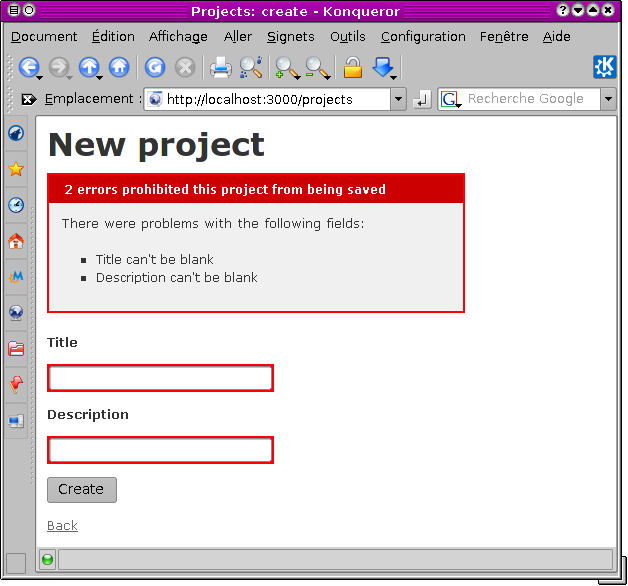
\includegraphics[width=60mm]{error_screenshot.png}
        \end{column}
    \end{columns}
\end{frame}

\begin{frame}
    \frametitle{Les associations}
    \begin{center}
        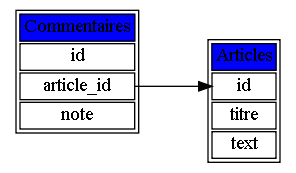
\includegraphics[width=40mm]{article_commentaire.png}
        \lstinputlisting[language=Ruby,numbers=left,basicstyle=\scriptsize]{article.rb}
    \end{center}
\end{frame}


\section{Composant Controller de Ruby On Rails}

\begin{frame}
    \frametitle{1 methode, 1 URL}
    \begin{itemize}
        \item Url implicite à partir du nom de controlleur et du nom de la
        methode
        \item Utilisation de routes nommée
        \item Définission implicite du fichier de Vue
    \end{itemize}
\end{frame}

\begin{frame}
    \frametitle{RESTFULL}

    \begin{itemize}
        \item REST (Representational State Transfer)
        \item Basé sur les 4 Verbes HTTP~:
            \begin{itemize}
                \item POST (create)
                \item GET (show)
                \item PUT (update)
                \item DELETE (delete)
            \end{itemize}
        \item Utilisation des verbes simples avec URL correspondant.
        \item Facilité de création d'une API
    \end{itemize}
\end{frame}

\begin{frame}
    \frametitle{Exemple de controller}
    \lstinputlisting[language=Ruby,numbers=left,basicstyle=\scriptsize]{project_controller.rb}
\end{frame}

\section{Composant de vue de Rails}

\begin{frame}
    \frametitle{Les helpers}

    \begin{itemize}
        \item 1 helper par controller par défaut
        \item réutilisation des manipulations de vues
        \item de nombreuses méthodes existantes dans l'API
    \end{itemize}
\end{frame}

\begin{frame}
    \frametitle{ActionView}
    \begin{block}{app/views/project/list.html.erb}
        \lstinputlisting[language=Ruby,numbers=left,basicstyle=\tiny,showspaces=false,showstringspaces=false]{list.html.erb}
    \end{block}
    \begin{block}{app/views/project/show.html.erb}
        \lstinputlisting[language=Ruby,numbers=left,basicstyle=\tiny,showspaces=false,showstringspaces=false]{show.html.erb}
    \end{block}
    \begin{block}{app/views/task/\_task.html.erb}
        \lstinputlisting[language=Ruby,numbers=left,basicstyle=\tiny,showspaces=false,showstringspaces=false]{_task.html.erb}
    \end{block}
\end{frame}


\section{Les tests}

\begin{frame}
    \frametitle{Les tests unitaires}
    \begin{itemize}
        \item Dans le dossier /test/units
        \item Test sur les classes models
        \item Facilité de créer un jeux de test
        \item Base de donnée indépendante
        \item Réinjection automatique des données à chaques tests
    \end{itemize}
\end{frame}

\begin{frame}
    \frametitle{Les test fonctionnels}
    \begin{itemize}
        \item Dans le dossier /test/functionals
        \item Test sur les controlleurs
        \item Même système d'injection des jeux de données
        \item assertion spécifique avec vérification du DOM
    \end{itemize}
\end{frame}

\end{document}
